\documentclass[pdf,t]{beamer}
\newcommand\REV{v1.1.1}
% Berlin Berkeley Warsaw
\newcommand\z[1]{\texttt{#1}}
\usepackage{listings}
\usepackage{xeCJK}
\newcommand\identifier[1]{{\color{green!70!black}\z{#1}}}
\newcommand\keyword[1]{{\color{blue}\z{#1}}}
\newcommand\blocked[1]{{\color{red}\z{#1}}}
\newcommand\gostring[1]{{\color{orange!90!black}\z{#1}}}
\newcommand\playground[1]{\framebox{\color{gray}\z{https://go.dev/play/#1}}}
\lstset{
    language=Go,
    basicstyle=\ttfamily,
    keywordstyle=\color{blue}\ttfamily\bfseries,
    identifierstyle=\color{green!70!black},
    commentstyle=\ttfamily\color{gray},
    stringstyle=\ttfamily\color{orange!90!black},
    showstringspaces=false
}
\mode<presentation>{\usetheme{Berlin}\useoutertheme{infolines}\useinnertheme{rounded}}
\title{A Whirlwind Tour of Go}
\subtitle{Just the Cool Parts}
\author{Steve Willoughby}
\date{15-Apr-2024\\{\tiny\REV}}
\begin{document}
\begin{frame}
    \titlepage
    \begin{center}
    
\includegraphics[height=.25\textheight]{go-logo}
    
\includegraphics[height=.25\textheight]{gopher}
    \end{center}
\end{frame}
\section[Overview]{Overview}
\subsection{What Are We Doing Here?}
\begin{frame}{The Point}
    \begin{itemize}
        \item ``What \emph{is} Go?''
        \item ``What is it actually good for?''
        \item ``Why should I care?''
    \end{itemize}
\end{frame}
\subsection{Motivation for Go}
\begin{frame}{30 Seconds of History}
    \begin{itemize}
        \item Designed by Rob Pike, Ken Thompson, and Robert Griesemer.
        \item Includes direct experience with C from day 1 to now.
            \pause
        \item ``If we were to design C today, knowing what we know now, on today's technology\dots''
            \pause
            \begin{itemize}
        \item $\therefore$ Go's syntax is very much like C's
        \item \dots\ but cleaned up and streamlined a bit.
            \end{itemize}
        \pause
    \item Dreamed up while waiting on a 45-minute C\texttt{++} compile
        \pause
            \begin{itemize}
                \item Fast compilation
                \item Native binary compiler with low overhead
                \item Strong static typing
                \item Extraordinarily spartan
            \end{itemize}
    \end{itemize}
\end{frame}
\section{Introducing Go}
\begin{frame}[c]{The Basics}
	\begin{center}
	\Huge This is the ``whirlwind'' part\dots

		\bigskip

	\Large (Laying a foundation of the basics so the more interesting discussions are understandable.)
	\end{center}
\end{frame}
\subsection{The Basics}
\begin{frame}{Intrinsic Data Types}
    \begin{itemize}
        \item The usual suspects: 
            \keyword{int}, 
            \keyword{int8}, 
            \keyword{int16}, 
            \keyword{int32}, 
            \keyword{int64}, 
            \keyword{uint}, 
            \keyword{uint8}, 
            \keyword{uint16}, 
            \keyword{uint32}, 
            \keyword{uint64}, 
            \keyword{bool},
            \keyword{byte},
            \keyword{float32},
            \keyword{float64},
            \keyword{string}.
            \begin{itemize}
                \item \gostring{"hello"}, \gostring{`hello`}, \z{42}, \z{0x7F}, \z{0o177}, \z{0b11010111}
            \end{itemize}
            \pause
        \item Special things:
            \keyword{complex64},
            \keyword{complex128},
            \keyword{error}.
            \begin{itemize}
                \item \z{13+2i}, \identifier{complex}\z{(13, 2)}
            \end{itemize}
            \pause
        \item Structures: \keyword{struct}\z{\{}\dots\z{\}}.
            \pause
        \item What about \keyword{char}? Nope. Instead, we have \keyword{rune}.
            \begin{itemize}
                \item \gostring{'A'}, \gostring{'\textbackslash n'}, \gostring{'$\Sigma$'}
            \end{itemize}
            \pause
        \item Arrays: \z{[10]}\keyword{int}, \z{[100]}\keyword{rune}.
            \pause
        \item Slices: \z{[]}\keyword{int}, \z{[]}\keyword{byte}, \z{[]}\keyword{string}.
            \pause
        \item Maps: \keyword{map}\z{[}\keyword{string}\z{]}\keyword{int}.
            \pause
        \item Channels: \keyword{chan int}.
    \end{itemize}
\end{frame}

\begin{frame}{Expressions and Operators}
    \begin{itemize}
        \item Arithmetic:
            \z{+},
            \z{-},
            \z{*},
            \z{/},
            \z{\%}.
        \item Relational:
            \z{==},
            \z{!=},
            \z{>},
            \z{<},
            \z{>=},
            \z{<=}.
        \item Logical:
            \z{\&\&},
            \z{||},
            \z{!}.
        \item Bitwise:
            \z{\&},
            \z{|},
            \z{\textasciicircum},
            \z{<<},
            \z{>>},
            \z{\&\textasciicircum}.
            \hfill\z{// }\identifier{x}\z{ \&\textasciicircum\ }\identifier{y}\z{ == }\identifier{x}\z{ \& (\textasciicircum}\identifier{y}\z{)}
        \pause
        \item Assignment:
            \z{=},
            \z{+=},
            \z{-=},
            \z{*=},
            \z{/=},
            \z{\%=},
            \z{\&=},
            \z{\textasciicircum=},
            \z{|=},
            \z{<<=},
            \z{>>=},
            \z{:=}.
        \pause
        \item Reference/Dereference: \z{\&}, \z{*}.
        \item Unary: \z{+}, \z{-}, \z{\textasciicircum}. \hfill\z{// \textasciicircum}\identifier{x}
        \item Increment/Decrement: \z{++}, \z{-{}-}. \hfill\z{// }\identifier{x}\z{++} or \identifier{x}\z{-{}-}
        \pause
        \item Channel I/O: \z{<-}. \hfill\z{// }\identifier{channel}\z{<-}\identifier{x} or \z{<-}\identifier{channel}
        \pause
        \item Blank identifier: \identifier{\_}.
    \end{itemize}
\end{frame}

\begin{frame}[fragile]{Declarations}
    \begin{itemize}
        \item Type declarations \emph{follow} identifier names
\begin{lstlisting}
var x int
var UserName string
\end{lstlisting}
\pause
\begin{lstlisting}
func AddNumbers(x, y int) int { ... }
func DivideNumbers(x, y int) (int, error) { ... }
\end{lstlisting}
\pause
\begin{lstlisting}
type Shape struct {
   X     int
   Y     int
   Color ColorCode
}
\end{lstlisting}
    \end{itemize}
\end{frame}
\begin{frame}{Program Structure}
    \begin{itemize}
        \item Basic unit is a \emph{package} (namespace boundary).\pause
        \item Multiple source files in a package, in the same directory.\pause
        \item Every program must have a \identifier{main} package.
        \item The \identifier{main} package has a \identifier{main} function.\pause
        \item Import packages into the program using the \keyword{import} statement.
        \item Always prefix identifiers from imported packages with their package name.\pause
        \item Identifiers can be \emph{public} or \emph{private} w/r/t package boundaries.\pause
            \begin{itemize}
                \item Identifier names starting with an uppercase letter are public.
                \item All others are private.
            \end{itemize}
    \end{itemize}
\end{frame}

\begin{frame}[fragile]{Hello, World}
\playground{}
\begin{lstlisting}
/* Standard-issue "Hello, World" program in Go */

package main

import "fmt"

func main() {
     fmt.Println("Hello, 世界")
}
\end{lstlisting}
\end{frame}
\subsection{The Go Ecosystem}
\begin{frame}{The Playground}
    \begin{itemize}
        \item Interactive playground to immediately try something in Go.
        \item \z{https://go.dev/play/}
    \end{itemize}
    \begin{center}
        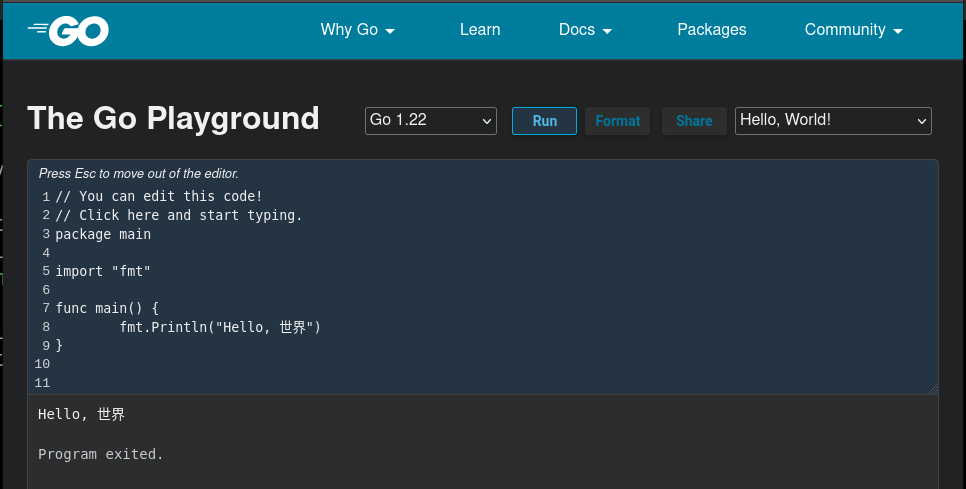
\includegraphics[width=\textwidth]{playground}
    \end{center}
\end{frame}
\begin{frame}[fragile]{Importing Third-Party Packages}
    \begin{itemize}
        \item Standard library package names are simple names:
            \begin{lstlisting}
import "fmt"
import "encoding/json"
import "flag"
import "math"
\end{lstlisting}
\pause
        \item Getting packages from public repositories:
\begin{lstlisting}
import "github.com/MadScienceZone/go-gma/v5/dice"
\end{lstlisting}
    \end{itemize}
    \vfill
    \strut
\end{frame}
\begin{frame}{Automatic API Documentation}
\begin{itemize}
\item\z{https://pkg.go.dev/}\emph{repository-url}
\end{itemize}
    \begin{center}
        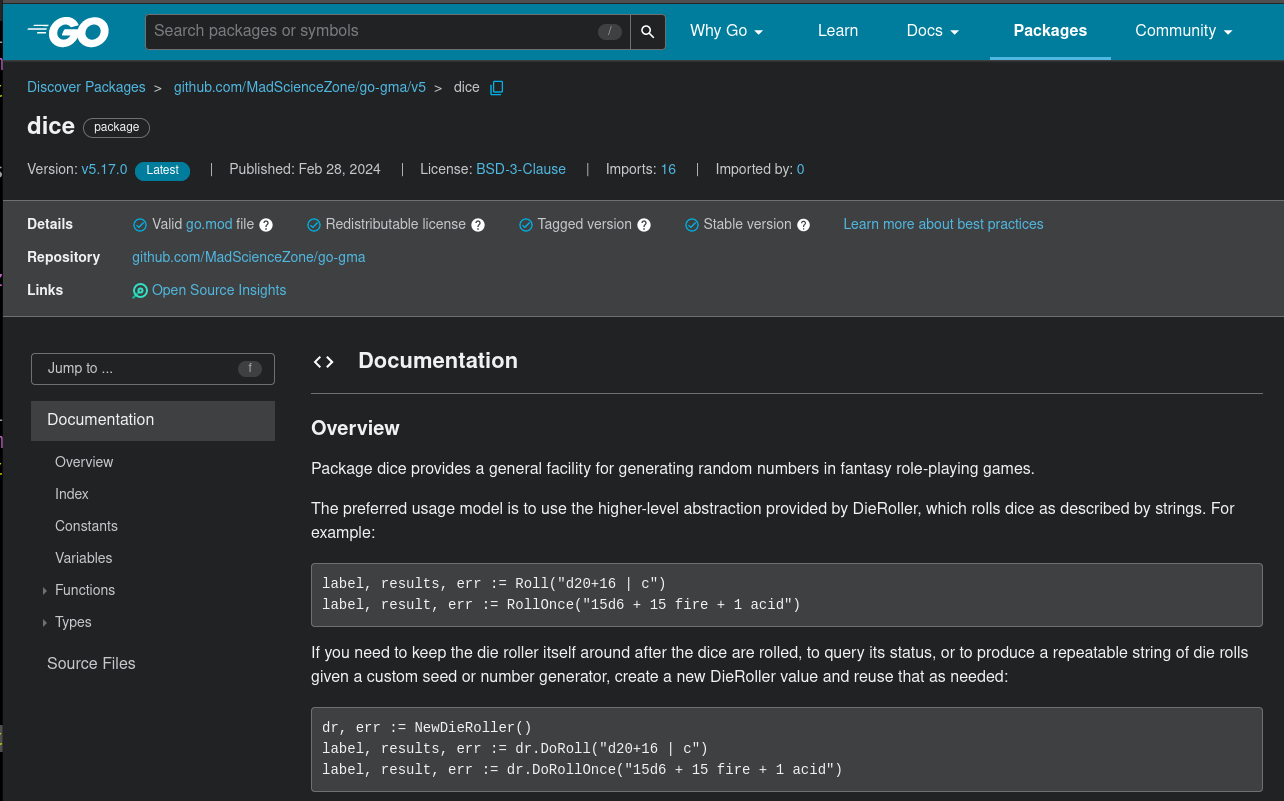
\includegraphics[width=\textwidth]{docsite}
    \end{center}
\end{frame}

\subsection{Go Syntax}
\begin{frame}[fragile]{``Factored'' Notation}
\begin{lstlisting}
import "fmt"
import "encoding/json"
import "flag"
import "math"
\end{lstlisting}
\pause
\begin{lstlisting}
import (
   "fmt"
   "encoding/json"
   "flag"
   "math"
)
\end{lstlisting}
\end{frame}

\begin{frame}[fragile]{``Factored'' Notation}
\begin{lstlisting}
var initialized bool
var userNames   []string
var Greeting    string   = "Hello"
var TheAnswer            = 42
\end{lstlisting}
\begin{lstlisting}
var (
    initialized bool
    userNames   []string
    Greeting    string   = "Hello"
    TheAnswer            = 42
)
\end{lstlisting}
\end{frame}

\begin{frame}[fragile]{``Factored'' Notation}
\begin{lstlisting}
const initialized      = false
const Greeting         = "Hello"
const TheAnswer   byte = 42
\end{lstlisting}
\begin{lstlisting}
const (
    initialized      = false
    Greeting         = "Hello"
    TheAnswer   byte = 42
)
\end{lstlisting}
\end{frame}

\begin{frame}[fragile]{``Factored'' Notation and iota}
\begin{onlyenv}<1->
\playground{p/LSHu1VKUz20}
\begin{lstlisting}
type MessageType byte
const (
    ServerCommand MessageType = 0
    ServerReply   MessageType = 1
    ServerError   MessageType = 2
    UrgentMessage MessageType = 3
)
\end{lstlisting}
\end{onlyenv}
\begin{onlyenv}<2>
\begin{lstlisting}
const (
    ServerCommand MessageType = iota
    ServerReply   MessageType = iota
    ServerError   MessageType = iota
    UrgentMessage MessageType = iota
)
\end{lstlisting}
\end{onlyenv}
\begin{onlyenv}<3>
\begin{lstlisting}
const (
    ServerCommand MessageType = iota
    ServerReply   
    ServerError   
    UrgentMessage 
)
\end{lstlisting}
\end{onlyenv}
\end{frame}
\begin{frame}[fragile]{``Factored'' Notation and iota Expressions}
\playground{p/LSHu1VKUz20}
\begin{lstlisting}
type MessageType byte
const (
    ServerCommand MessageType = 0x01
    ServerReply   MessageType = 0x02
    ServerError   MessageType = 0x04
    UrgentMessage MessageType = 0x08
)
\end{lstlisting}
\begin{lstlisting}
const (
    ServerCommand MessageType = 1 << iota
    ServerReply   
    ServerError   
    UrgentMessage 
)
\end{lstlisting}
\end{frame}

\subsection{Control Flow}
\begin{frame}[fragile]{Conditionals}
\begin{lstlisting}
var x int

if x > 10 {
    fmt.Println("X exceeds 10.")
} else {
    fmt.Println("X is tiny.")
}
\end{lstlisting}
\pause
\begin{lstlisting}
if x *= 2; x > 10 {
    fmt.Println("Now X is big.")
} else {
    fmt.Println("X is still small.")
}
\end{lstlisting}
\end{frame}
\begin{frame}[fragile]{Switches}
\begin{lstlisting}
var x int

switch x {
case 0:
    fmt.Println("X is nothing.")
case 1, 3, 5:
    fmt.Println("X is odd.")
case 2, 4, 6:
    fmt.Println("X is even.")
default:
    fmt.Println("X is bigger than I can count.")
}
\end{lstlisting}
\end{frame}
\begin{frame}[fragile]{Loops}
\begin{lstlisting}
// infinite loop
for {
}

// while loop
for thing.IsReady() {
}

// traditional 3-part for loop
for i := 0; i < 10; i++ {
}
\end{lstlisting}
\end{frame}

\begin{frame}[fragile]{Loops}
\begin{lstlisting}
// loop over interval [0,10)
for i := range 10 {
}

// loop over elements of a collection
for i, v := range []int{1, 4, -3, 153} {
}

// loop over data received from channel
for item := range channel {
}
\end{lstlisting}
\end{frame}


\subsection{Collection Types}
\begin{frame}[fragile]{Arrays}
    \begin{itemize}
        \item The number of elements \emph{is part of the type} (\z{[10]}\keyword{int} vs.\@ \z{[15]}\keyword{int}).
            \pause
        \item Variables declared are initialized empty but ready for use
\begin{lstlisting}
var things [5]string

things[0] = "raindrops on roses"
things[1] = "whiskers on kittens"
things[2] = "copper kettles"
things[3] = "woolen mittens"
things[4] = "wild geese"

fmt.Println("I like", things[2])
fmt.Println("I also like", things)
fmt.Println("I know", len(things), "things.")
\end{lstlisting}
    \end{itemize}
\end{frame}

\begin{frame}[fragile]{Arrays}
    \playground{p/rexZjp6SdKD}
    \begin{itemize}
        \item Or you can specify an array literal value to use in an expression or assign to a variable
\begin{lstlisting}
things := [5]string{
    "raindrops on roses",
    "whiskers on kittens",
    "copper kettles",
    "woolen mittens",
    "wild geese",
}

fmt.Println("I like", things[2])
fmt.Println("I also like", things)
fmt.Println("I know", len(things), "things.")
\end{lstlisting}
    \end{itemize}
\end{frame}

\begin{frame}[fragile]{Slices}
    \playground{p/rexZjp6SdKD}
    \begin{itemize}
        \item Specify a range \z{[}$n$\z{:}$m$\z{]} as the index into an array to get a subset of the array values
            with indices from $n$ to $m-1$.
        \item The value is a \emph{slice}, not an \emph{array}. It's a different type.
        \begin{itemize}
            \item For \z{[5]}\keyword{string}, the value is \z{[]}\keyword{string}.
        \end{itemize}
    \end{itemize}
\begin{lstlisting}
fmt.Println("Some things:", things[1:3])
fmt.Println("Some things:", things[:3])
fmt.Println("Some things:", things[1:])
fmt.Println("Some things:", things[:])
\end{lstlisting}
\end{frame}
\begin{frame}[fragile]{Slices}
    \playground{p/rexZjp6SdKD}
    \begin{itemize}
        \item Dimensionless ``arrays'': \z{[]}\keyword{int}.
        \item Actually a ``view'' into an underlying array.
            \begin{itemize}
                \item Go creates and manages the underlying array automatically for you.
            \end{itemize}
    \end{itemize}
\begin{lstlisting}
var things []string
\end{lstlisting}
\pause
\begin{lstlisting}
things = append(things, "doorbells")
things = append(things, "sleighbells", "schnitzel")
fmt.Println(len(things), things) 
// prints:  3 [doorbells sleighbells schnitzel]
\end{lstlisting}
\end{frame}

\begin{frame}[fragile]{Slices}
    \playground{p/rexZjp6SdKD}
    \begin{itemize}
        \item Can also specify a slice of values as a literal.
    \end{itemize}
\begin{lstlisting}
things := []string{
    "doorbells",
    "sleighbells",
    "schnitzel",
}
\end{lstlisting}
\pause
\begin{lstlisting}
primes := []int{2, 3, 5, 7, 11, 13}
lowPrimes := slices.Delete(primes, 3, len(primes))
fmt.Println(lowPrimes)
// prints:  [2 3 5]
\end{lstlisting}
\end{frame}

\begin{frame}[fragile]{Maps}
\playground{p/Bfs6kEUKwve}
\begin{lstlisting}
var Ages map[string]int
Ages = make(map[string]int)
\end{lstlisting}
\pause
\begin{lstlisting}
Ages["Alice"] = 14
Ages["Bob"] = 22
Ages["Charlie"] = 27
Ages["Daria"] = 42
fmt.Println(Ages)
\end{lstlisting}
\end{frame}
\begin{frame}[fragile]{Maps}
\playground{p/Bfs6kEUKwve}
\begin{lstlisting}
Ages := map[string]int{
    "Alice": 14,
    "Bob": 22,
    "Charlie": 27,
    "Daria": 42,
}
fmt.Println(Ages)
\end{lstlisting}
\begin{lstlisting}
for name, age := range Ages {
    if age >= 18 {
        fmt.Printf("%s may vote.\n", name)
    } else {
        fmt.Printf("%s is not eligible.\n", name)
    }
}
\end{lstlisting}
\end{frame}
\begin{frame}[fragile]{Maps}
\playground{p/Bfs6kEUKwve}
\begin{onlyenv}<1->
\begin{lstlisting}
aliceAge := Ages["Alice"]      // 14
eveAge := Ages["Eve"]          // 0
\end{lstlisting}
\end{onlyenv}
\begin{onlyenv}<2->
\begin{lstlisting}
aliceAge, exists := Ages["Alice"]      // 14, true
eveAge, exists := Ages["Eve"]          // 0, false
\end{lstlisting}
\end{onlyenv}
\begin{onlyenv}<3->
\begin{lstlisting}
Ages["Eve"] = 20
delete(Ages, "Bob")
\end{lstlisting}
\end{onlyenv}
\begin{onlyenv}<4>
\begin{lstlisting}
if _, exists := Ages[name]; exists {
    fmt.Prinln("We do know about", name)
}
\end{lstlisting}
\end{onlyenv}
\begin{onlyenv}<5>
\begin{lstlisting}
if age, exists := Ages[name]; exists {
    fmt.Printf("We know %s's age is %d.\n", name, age)
} else {
    fmt.Println("We don't know", name)
}
\end{lstlisting}
\end{onlyenv}
\end{frame}

\subsection{Error Handling}
\begin{frame}[c]{Error Values}
	\begin{center}
	\Huge Error Handling
	\end{center}
\end{frame}
\begin{frame}[fragile]{Error Values}
\begin{lstlisting}
func main() {
    var intval int
    var err    error

    for i, arg := range os.Args[1:] {
        intval, err = strconv.Atoi(arg)
        if err != nil {
            fmt.Printf("Arg #%d (\"%s\"): %v.\n",
                       i, arg, err)
        } else {
            fmt.Printf("Arg #%d == %d\n", i, intval)
        }
    }
}
\end{lstlisting}
\end{frame}
\section{What Makes Go Different}
\begin{frame}[c]{Object Oriented Features}
	\begin{center}
	\Huge Wherewith Object Orientation?

		\bigskip

		\Large (For a language without object classes\dots)
	\end{center}
\end{frame}

\subsection{Object Oriented Features}
\begin{frame}[fragile]{Structures}
\playground{p/TClHUvPovi0}
\begin{lstlisting}
type Triangle struct {
    Base   int
    Height int
    X      int // Reference point
    Y      int
}
\end{lstlisting}
\begin{onlyenv}<2>
\begin{lstlisting}
var t1 Triangle
t1.Base = 37
t1.Height = 15
t1.X = 11
t1.Y = 22
\end{lstlisting}
\end{onlyenv}
\begin{onlyenv}<3>
\begin{lstlisting}
var t2 Triangle = Triangle{Base: 3, Height: 1}

fmt.Println("t2's base is", t2.Base)
\end{lstlisting}
\end{onlyenv}
\begin{onlyenv}<4>
\begin{lstlisting}
t3 := Triangle{
    Base:   100,
    Height: 42,
    X:      -3,
    Y:      14,
}
\end{lstlisting}
\end{onlyenv}
\end{frame}

\begin{frame}[fragile]{Method Functions}
\playground{p/TClHUvPovi0}
\begin{lstlisting}
func Area(t Triangle) float64 {
    return (float64(t.Base) * 
            float64(t.Height)) / 2.0
}

func Translate(t Triangle, dx, dy int) Triangle {
    t.X += dx
    t.Y += dy
    return t
}

fmt.Println("t1 area =", Area(t1))
t2 = Translate(t2, +3, -2)
\end{lstlisting}
\end{frame}

\begin{frame}[fragile]{Method Functions}
\playground{p/TClHUvPovi0}
\begin{lstlisting}
func Area(t Triangle) float64 {
    return (float64(t.Base) * 
            float64(t.Height)) / 2.0
}

func Translate(t *Triangle, dx, dy int) {
    t.X += dx
    t.Y += dy
}

fmt.Println("t1 area =", Area(t1))
Translate(&t2, +3, -2)
\end{lstlisting}
\end{frame}

\begin{frame}[fragile]{Method Functions}
\playground{p/TClHUvPovi0}
\begin{lstlisting}
func (t Triangle) Area() float64 {
    return (float64(t.Base) * 
            float64(t.Height)) / 2.0
}

func (t *Triangle) Translate(dx, dy int) {
    t.X += dx
    t.Y += dy
}

fmt.Println("t1 area =", t1.Area())
t2.Translate(+3, -2)
\end{lstlisting}
\end{frame}

\begin{frame}[fragile]{Composition}
\playground{p/qp2nc6gywLr}
\begin{lstlisting}
type BaseShape struct {
    X int
    Y int
}

func (s BaseShape) ReferencePoint() (int, int) {
    return s.X, s.Y
}

// (We'll set aside the Translate method for now to
// keep the in-class example simple.)
\end{lstlisting}
\end{frame}

\begin{frame}[fragile]{Composition}
\playground{p/qp2nc6gywLr}
\begin{lstlisting}
type Triangle struct {
    BaseShape
    Base   int
    Height int
}

func (t Triangle) Area() float64 {
    return (float64(t.Base) * 
            float64(t.Height)) / 2.0
}
\end{lstlisting}
\end{frame}

\begin{frame}[fragile]{Composition}
\playground{p/qp2nc6gywLr}
\begin{lstlisting}
type Rectangle struct {
    BaseShape
    Width  int
    Height int
}

func (r Rectangle) Area() float64 {
    return float64(r.Width * r.Height)
}
\end{lstlisting}
\end{frame}

\begin{frame}[fragile]{Composition}
\playground{p/qp2nc6gywLr}
\begin{lstlisting}
// Regular Polygons
type Polygon struct {
    BaseShape
    Sides  int
    Length float64  // Length of each side
    Radius float64  // Radius of inscribed circle
}

func (p Polygon) Area() float64 {
    return (float64(p.Sides) / 2.0) *
            p.Length * p.Radius
}
\end{lstlisting}
\end{frame}

\begin{frame}[fragile]{Composition}
\playground{p/qp2nc6gywLr}
\begin{lstlisting}
type Circle struct {
    BaseShape
    Radius float64
}

func (c Circle) Area() float64 {
    return math.Pi * math.Pow(c.Radius, 2)
}
\end{lstlisting}
\end{frame}
\begin{frame}[fragile]{Composition}
\playground{p/qp2nc6gywLr}
\begin{lstlisting}
c := Circle{
    BaseShape: BaseShape{
        X: 1, 
        Y: 2,
    }, 
    Radius: 1.5,
}
\end{lstlisting}
\pause
\begin{lstlisting}
fmt.Println(c.BaseShape.X, c.BaseShape.Y, 
            c.Radius, c.Area())
\end{lstlisting}
\pause
\begin{lstlisting}
fmt.Println(c.X, c.Y, c.Radius, c.Area())
\end{lstlisting}
\end{frame}

\begin{frame}[fragile]{Polymorphism}
\playground{p/qp2nc6gywLr}
\begin{onlyenv}<1>
\begin{lstlisting}
shapes := []Shape{
    Triangle{
        BaseShape: BaseShape{
            X: 3, 
            Y: 12,
        }, 
        Base: 3, 
        Height: 2,
    },
    Circle{BaseShape:BaseShape{Y: 22}, Radius: 1.5},
    Rectangle{Height: 100, Width: 50},
}
\end{lstlisting}
\end{onlyenv}
\begin{onlyenv}<2>
\begin{lstlisting}
shapes := []Shape{
    Triangle{BaseShape: BaseShape{X: 3, Y: 12}, 
        Base: 3, Height: 2},
    Circle{BaseShape:BaseShape{Y: 22}, Radius: 1.5},
    Rectangle{Height: 100, Width: 50},
}

for i, shape := range shapes {
    x, y := shape.ReferencePoint()
    fmt.Printf("#%d at (%d,%d), area=%f\n",
               i, x, y, shape.Area())
}
\end{lstlisting}
\end{onlyenv}
\end{frame}

\begin{frame}[fragile]{Polymorphism via Interfaces}
\playground{p/qp2nc6gywLr}
\begin{lstlisting}
type Shape interface {
    Area() float64
    ReferencePoint() (int, int)
}
\end{lstlisting}
\pause
\begin{lstlisting}
func reportArea(s Shape) {
    fmt.Printf("The area is %f\n", s.Area()
}
\end{lstlisting}
\end{frame}

\begin{frame}[c]{Type Assertions}
	\begin{center}
	\Huge Type Assertions
	\end{center}
\end{frame}
\begin{frame}[fragile]{Type Assertions}
\playground{p/dy952C3yZUX}
\begin{onlyenv}<1-2>
\begin{lstlisting}
f(42)
f(-2)
\end{lstlisting}
\end{onlyenv}
\begin{onlyenv}<3->
\begin{lstlisting}
f(42)
f("hello")
\end{lstlisting}
\end{onlyenv}
\begin{lstlisting}
func f(mystery any) {    // any == interface{}
    var v int
\end{lstlisting}
\begin{onlyenv}<1>
\begin{lstlisting}
    // we know it's an int, just treat it as one
    v = mystery + 15
\end{lstlisting}
\end{onlyenv}
\begin{onlyenv}<2-3>
\begin{lstlisting}
    x := mystery.(int)
    v = x + 15
\end{lstlisting}
\end{onlyenv}
\begin{onlyenv}<4>
\begin{lstlisting}
    x, ok := mystery.(int)
    v = x + 15
\end{lstlisting}
\end{onlyenv}
\begin{lstlisting}
    fmt.Println("int mystery is", v)
}
\end{lstlisting}
\end{frame}

\begin{frame}[fragile]{Type Switch}
\playground{p/dy952C3yZUX}
\begin{lstlisting}
f(42)
f("hello")
func f(mystery any) {    // any == interface{}
    var v int
    
    switch x := mystery.(type) {
    case int:
        v = x + 15
    case string:
        fmt.Println("string", x)
    default:
        // handle the unknown type
    }
}
\end{lstlisting}
\end{frame}

\subsection{Concurrency}
\begin{frame}[c]{Goroutines}
	\begin{center}
	\Huge Concurrency!
	
		\bigskip

	\Large (Goroutines and Channels and some other things)
	\end{center}
\end{frame}
\begin{frame}[fragile]{Goroutines---Calling a Function in the ``Background''}
\playground{p/FJNbOcNYI8-}
\begin{lstlisting}
func countdown() {
    for i := 10; i >= 0; i-- {
        fmt.Printf(">>> %d <<<\n", i)
        time.Sleep(1 * time.Second)
    }
}
\end{lstlisting}
\pause
\begin{lstlisting}
func main() {
    countdown()
    fmt.Println("Starting a long-running task...")
    time.Sleep(15 * time.Second)
    fmt.Println("Done. Exiting.")
}
\end{lstlisting}
\end{frame}

\begin{frame}[fragile]{Goroutines---Calling a Function in the ``Background''}
\playground{p/FJNbOcNYI8-}
\begin{lstlisting}
func countdown() {
    for i := 10; i >= 0; i-- {
        fmt.Printf(">>> %d <<<\n", i)
        time.Sleep(1 * time.Second)
    }
}
\end{lstlisting}
\begin{lstlisting}
func main() {
    go countdown()
    fmt.Println("Starting a long-running task...")
    time.Sleep(15 * time.Second)
    fmt.Println("Done. Exiting.")
}
\end{lstlisting}
\end{frame}


\begin{frame}[fragile]{Channels}
\playground{p/sFuhOuwVS6c}
\begin{lstlisting}
ch := make(chan byte)
\end{lstlisting}
\pause
\begin{lstlisting}
fmt.Println("Writing to channel")
\end{lstlisting}
\identifier{ch}\z{ <- 42}
\begin{lstlisting}
fmt.Println("Reading from channel")
x := <-ch
fmt.Println("Read", x, "from channel")
\end{lstlisting}
\end{frame}

\begin{frame}[fragile]{Channels}
\playground{p/sFuhOuwVS6c}
\begin{lstlisting}
ch := make(chan byte)
\end{lstlisting}
\begin{lstlisting}
fmt.Println("Writing to channel")
\end{lstlisting}
{\color{red}\z{ch <- 42\qquad\qquad// DEADLOCKED!}}
\begin{lstlisting}
fmt.Println("Reading from channel")
x := <-ch
fmt.Println("Read", x, "from channel")
\end{lstlisting}
\end{frame}

\begin{frame}[fragile]{Channels}
\playground{p/sFuhOuwVS6c}
\begin{lstlisting}
ch := make(chan byte)
go func(c chan byte) {
    x := <-c
    fmt.Println("Read", x, "from channel")
}(ch)

fmt.Println("Writing to channel")
ch <- 42
\end{lstlisting}
\end{frame}

\begin{frame}[fragile]{Buffered Channels}
\playground{p/sFuhOuwVS6c}
\begin{lstlisting}
ch := make(chan byte, 1)
\end{lstlisting}
\pause
\begin{lstlisting}
fmt.Println("Writing to channel")
ch <- 42

fmt.Println("Reading from channel")
x := <-ch
fmt.Println("Read", x, "from channel")
\end{lstlisting}
\end{frame}


\begin{frame}[c]{Select}
	\begin{center}
	\Huge Select
	\end{center}
\end{frame}

\begin{frame}[fragile]{Select (C)}
\begin{lstlisting}[language=c]
#include <sys/select.h>
fd_set read_handles, write_handles, err_handles;
struct timeval t;
int sel = 0;

FD_ZERO(&read_handles);
FD_ZERO(&write_handles);
FD_ZERO(&err_handles);
/* set bits for handles you're interested in */
t.tv_sec = 1;
t.tv_usec = 0;
\end{lstlisting}
\end{frame}
\begin{frame}[fragile]{Select (C)}
\begin{lstlisting}[language=c]
if ((sel = select(maxfd, &read_handles, 
                  &write_handles, 
                  &err_handles, &t)) == -1) {
    /* error... */
}
else if (sel > 0) {
    /* go back and check the bits in *_handles */
}
\end{lstlisting}
\end{frame}
\begin{frame}[fragile]{Select (Go)}
\begin{lstlisting}
select {
case x := <-ichan:
    // we could read from ichan, proceed
    // with that...

case ochan <- ovalue:
    // we could write to ochan
\end{lstlisting}
\begin{onlyenv}<2>
\begin{lstlisting}
default:
    // if we don't want the whole select to
    // block, add a default case here.
\end{lstlisting}
\end{onlyenv}
\begin{lstlisting}
}
\end{lstlisting}
\end{frame}


\subsection{Thread-Safe Memory Access}
\begin{frame}[c]{Global ID Generation Examples}
	\begin{center}
	\Huge Thread-Safe Memory Access

		\bigskip

	\Large by example
	\end{center}
\end{frame}
\begin{frame}[fragile]{Global ID Generation (Na\"\i ve)}
\playground{p/iOxsFX\_TSaa}
\begin{lstlisting}
type GameState struct {
    NextMessageID int
}
\end{lstlisting}

\begin{onlyenv}<2>
\begin{lstlisting}
var gameserver GameState

// In many concurrent goroutines...
\end{lstlisting}
\identifier{gameServer}\z{.}\identifier{NextMessageID}\z{++}\\
\identifier{client}\z{.}\identifier{ID}\z{ = }\identifier{gameServer}\z{.}\identifier{NextMessageID}
\end{onlyenv}
\begin{onlyenv}<3>
\begin{lstlisting}
var gameserver GameState

// In many concurrent goroutines...
\end{lstlisting}
{\color{red}\z{gameServer.NextMessageID++~~~~~~~~~~~~~~~~// UNSAFE!}\\
\z{client.ID = gameServer.NextMessageID~~~~~~// UNSAFE!}}
\end{onlyenv}
\end{frame}

\begin{frame}[fragile]{Global ID Generation (Mutex)}
\playground{p/iOxsFX\_TSaa}
\begin{onlyenv}<1->
\begin{lstlisting}
type GameState struct {
    nextMessageID int
    lock          sync.Mutex
}
\end{lstlisting}
\end{onlyenv}
\begin{onlyenv}<1>
\begin{lstlisting}
func (state *GameState) GetNextID() int {





}
\end{lstlisting}
\end{onlyenv}
\begin{onlyenv}<2>
\begin{lstlisting}
func (state *GameState) GetNextID() int {
    state.lock.Lock()
    state.nextMessageID++
    nextID := state.MessageID
    state.lock.Unlock()
    return nextID
}
\end{lstlisting}
\end{onlyenv}
\begin{onlyenv}<3>
\begin{lstlisting}
func (state *GameState) GetNextID() int {
    state.lock.Lock()
    defer state.lock.Unlock()

    state.nextMessageID++
    return state.nextMessageID
}
\end{lstlisting}
\end{onlyenv}
\begin{onlyenv}<1->
\begin{lstlisting}
// in many random goroutines...
client.ID = gameServer.GetNextID()
\end{lstlisting}
\end{onlyenv}
\end{frame}

\begin{frame}[fragile]{Global ID Generation (Mutex)}
\playground{p/iOxsFX\_TSaa}
\begin{lstlisting}
func main() {
    var gameServer GameState
    var wg         sync.WaitGroup
    for i := range 100 {
        wg.Add(1)
        id := i
        go func() {
            defer wg.Done()
            fmt.Printf("Goroutine #%d, ID=%d\n", id, 
                       gameServer.GetNextID())
        }()
    }
    wg.Wait()
}
\end{lstlisting}
\end{frame}
    

\begin{frame}[c]{Global ID Generation (Channel)}
	\begin{center}
	\Huge But that's not very idiomatic for Go.

	\bigskip

		\Large Here's a much better approach\dots
	\end{center}
\end{frame}
\begin{frame}[fragile]{Global ID Generation (Channel)}
\playground{p/mRfglxbH-kI}
\begin{lstlisting}
func serveMessageIDs(c chan<- int) {
    var id int
    for {
        c <- id
        id++
    }
}
\end{lstlisting}
\pause
\begin{lstlisting}
// start up the service
IDSource := make(chan int)
go serveMessageIDs(IDSource)
\end{lstlisting}
\pause
\begin{lstlisting}
// In many random goroutines...
client.ID = <-IDSource
\end{lstlisting}
\end{frame}

\section{Bonus/Backup Material}
\begin{frame}[c]{Bonus/Backup Material}
	\begin{center}
	\Huge Some more cool stuff if time allows\dots
	\end{center}
\end{frame}
\subsection{Contexts}
\begin{frame}[c]{Contextx}
	\begin{center}
	\Huge Contexts
	\end{center}
\end{frame}
\begin{frame}[fragile]{Contexts}
\playground{p/cPSNhVfS8r-}
\begin{lstlisting}
func collectData(stream <-chan string) error {
    for {
        data, ok := <-stream
        if !ok {
            return nil
        }
        if err := doSomething(data); err != nil {
            return err
        }
    }
}

// elsewhere
collectData(stream)
\end{lstlisting}
\end{frame}

\begin{frame}[fragile]{Contexts}
\playground{p/cPSNhVfS8r-}
\begin{lstlisting}
func collectData(ctx context.Context, 
                 stream <-chan string) error {
    for {
        select {
        case <-ctx.Done():
            return nil
        case data, ok := <-stream:
            if !ok { return nil }
            if err := doSomething(data); err != nil {
                return err
            }
        }
    }
}
\end{lstlisting}
\end{frame}

\begin{frame}[fragile]{Contexts}
\playground{p/cPSNhVfS8r-}
\begin{lstlisting}
// caller

ctx, cancel := context.WithTimeout(
    context.Background(), 5 * time.Second)
defer cancel()

if err := collectData(ctx, stream); err != nil {
    panic(err)
}
\end{lstlisting}
\end{frame}

\begin{frame}[fragile]{Contexts}
\playground{p/cPSNhVfS8r-}
\begin{lstlisting}
func collectData(ctx context.Context, 
                 stream <-chan string) error {
    for {
        select {
        case <-ctx.Done():
            return nil
        case <-time.After(2 * time.Second):
            log.Print("collectData taking too long")
        case data, ok := <-stream:   
            if !ok { return nil }
            if err := doSomething(data); err != nil {
                return err
            }
        }}}
\end{lstlisting}
\end{frame}

\subsection{JSON Encoding Made Easy}
\begin{frame}[c]{JSON}
	\begin{center}
		\Huge Encoding (JSON)
	\end{center}
\end{frame}
\subsection{JSON Encoding Made Easy}
\begin{frame}[fragile]{JSON}
\playground{p/\_KcMkqhhzbZ}
\begin{lstlisting}
import "encoding/json"
type User struct {
    Name   string   `json:"name"`
    ID     int      `json:",omitempty"`
    Attrs  []string `json:"attributes,omitempty"`
    Secret []byte   `json:"-"`
}
data := User{
    Name: "steve", 
    ID: 42, 
    Attrs: []string{"foo","bar"}, 
    Secret: sdata,
}
\end{lstlisting}
\end{frame}

\begin{frame}[fragile]{JSON}
\playground{p/\_KcMkqhhzbZ}
\begin{lstlisting}
import "encoding/json"

type User struct {
    Name   string   `json:"name"`
    ID     int      `json:",omitempty"`
    Attrs  []string `json:"attributes,omitempty"`
    Secret []byte   `json:"-"`
}

encoded, err := json.Marshal(data)
// {"name":"steve","ID":42,"attributes":["foo","bar"]}

var inputData User
err := json.Unmarshal(jsonBytes, &inputData)
\end{lstlisting}
\end{frame}
\section{}
\subsection{}
\begin{frame}{}
    \begin{center}
        
\includegraphics[height=.85\textheight]{gopher}
        \z{github.com/MadScienceZone/go-tour}
    \end{center}
\end{frame}
\end{document}
